\documentclass[conference]{IEEEtran}
\IEEEoverridecommandlockouts
\usepackage{cite}
\usepackage{amsmath,amssymb,amsfonts}
\usepackage{booktabs}
\usepackage{enumitem}
\usepackage{tikz}
\usetikzlibrary{arrows.meta,positioning}

\newcommand{\sat}{\operatorname{sat}}
\newcommand{\diag}{\operatorname{diag}}

\begin{document}

\title{Quanser QArm 4-DOF Manipulator:\\ Hardware Physics, Identification, Modelling, and the Complete Controller Suite\\
{\footnotesize Mathematical foundations for offline simulation, digital-twin, and hardware execution}}

\author{\IEEEauthorblockN{Gandhi Contreras}
\IEEEauthorblockA{\textit{Electrical and Computer Engineering}, New Mexico State University, Las Cruces, NM, USA \\ gandhico@nmsu.edu}}

\maketitle

\begin{abstract}
The QArm is a four-revolute-joint serial manipulator with a gripper, actuated by integrated ``smart servo'' modules that combine a DC motor, high-ratio gearing, an encoder, and an embedded drive with selectable position/velocity/current modes. This paper develops its complete mathematics: the smart-servo actuation physics and what high gear ratios do to reflected dynamics and backdrivability, the serial-chain kinematics (forward, inverse, Jacobian, singularities), the Euler--Lagrange dynamics with their structural properties, gravity loading and payload effects, identification of the base inertial parameters through the regressor formulation, and the controller suite --- joint PID with gravity compensation, LQR and LQG about operating configurations, computed-torque/backstepping, sliding mode, and NMPC --- together with the workspace, collision, and thermal safety envelope of an arm that shares space with people.
\end{abstract}

\begin{IEEEkeywords}
Serial manipulator, smart servos, Euler--Lagrange dynamics, inverse kinematics, computed torque, regressor identification, LQR, LQG, SMC, NMPC.
\end{IEEEkeywords}

%====================================================================
\section{Introduction}
Joint vector $q\in\mathbb R^4$ (base yaw, shoulder, elbow, wrist), gripper treated as an auxiliary axis. Kinematic structure: yaw about the vertical followed by a planar 2R chain (shoulder--elbow) and a wrist --- the anthropomorphic layout whose planar core admits closed-form inverse kinematics. The end-effector pose $x = f(q)$, Jacobian $J(q) = \partial f/\partial q$.

%====================================================================
\section{Hardware Physics}

\begin{figure*}[!t]
\centering
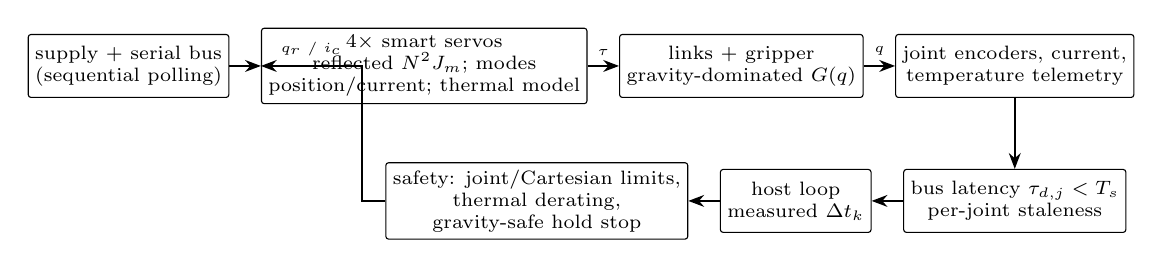
\begin{tikzpicture}[
  node distance=3mm and 4mm,
  blk/.style={draw, rounded corners=1pt, align=center, font=\scriptsize, inner sep=2.5pt, minimum height=8mm},
  lbl/.style={font=\tiny, align=center},
  arr/.style={-{Stealth[length=2mm]}, thick}
]

\node[blk] (sup) {supply + serial bus\\ (sequential polling)};
\node[blk, right=of sup] (srv) {$4\times$ smart servos\\ reflected $N^2J_m$; modes\\ position/current; thermal model};
\node[blk, right=of srv] (links) {links + gripper\\ gravity-dominated $G(q)$};
\node[blk, right=of links] (enc) {joint encoders, current,\\ temperature telemetry};
\node[blk, below=9mm of enc] (bus) {bus latency $\tau_{d,j} < T_s$\\ per-joint staleness};
\node[blk, left=of bus] (loop) {host loop\\ measured $\Delta t_k$};
\node[blk, left=of loop] (safe) {safety: joint/Cartesian limits,\\ thermal derating,\\ gravity-safe hold stop};
\draw[arr] (sup) -- (srv);
\draw[arr] (srv) -- node[lbl, above] {$\tau$} (links);
\draw[arr] (links) -- node[lbl, above] {$q$} (enc);
\draw[arr] (enc) -- (bus);
\draw[arr] (bus) -- (loop);
\draw[arr] (loop) -- (safe);
\draw[arr] (safe.west) -- ++(-3mm,0) |- node[lbl, pos=0.75, above] {$q_r$ / $i_c$} (srv.west);
\end{tikzpicture}
\caption{QArm signal chain: high-ratio smart servos dominate the reflected dynamics; the serial bus sets the outer loop rate; stops are gravity-safe position holds, never torque-free.}
\label{fig:chain}
\end{figure*}
\subsection{Smart-servo actuation}
Each joint is an integrated module: DC motor, gear train of ratio $N\!\sim\!10^2$, magnetic/optical encoder, temperature sensing, and an embedded controller with position, velocity, and current modes over a digital bus (half-duplex serial). The physics that dominate:
\begin{enumerate}[label=(\alph*)]
\item \emph{Reflected dynamics}: seen from the joint, rotor inertia and friction scale as $N^2 J_m$ and $N^2 b_m$ --- with $N\sim10^2$ the drivetrain contributes joint inertia comparable to the links and makes the joint effectively \emph{non-backdrivable}: external torques below the reflected breakaway do not move the motor. Consequences: excellent gravity holding for free, poor force transparency, and a plant whose diagonal (drivetrain) terms partially mask the configuration-dependent link coupling.
\item \emph{Mode physics}: in \emph{current mode} the module is a torque source $\tau = N k_t i_c$ (the assumption under which the dynamics-based controllers below act directly); in \emph{position/velocity mode} the embedded loop is part of the plant --- the outer controller commands setpoints through a servo lag, and torque is not directly assignable.
\item \emph{Bus latency}: the serial bus serves the joints sequentially; the loop period available to an outer controller is bus-bound (typically hundreds of hertz), and per-joint staleness enters as measurement delay.
\item \emph{Thermal envelope}: gravity holding is continuous $i^2R$ load; the embedded thermal model derates or shuts down --- sustained postures must respect the continuous-torque curve, not the peak.
\end{enumerate}

Manual-verified joint envelope (QArm): ranges base $\pm170^\circ$, shoulder $\pm85^\circ$, elbow $-95^\circ/{+}75^\circ$, wrist $\pm160^\circ$; maximum speed $\pi/2$~rad/s and acceleration $\pi/3$~rad/s$^2$ on every joint; instantaneous/continuous torque $10.6/2.65$ (base), $21.2/5.3$ (shoulder), $10.6/2.65$ (elbow), $4.1/1.0$ (wrist)~N\,m and $1.9/0.5$~N\,m (gripper), instantaneous limits permitted for at most $0.1$~s; motor temperature limit $50^\circ$C. The payload--endurance table ($350$~g indefinitely, $500$~g for $25{+}$~min, $750$~g for $15{+}$~min) is the thermal integral constraint of the NMPC formulation made empirical.

\subsection{Sensing and safety}
Joint encoders (absolute within the servo), currents and temperatures over the bus; no wrist force/torque sensor --- interaction forces are \emph{estimated} from currents through the gear efficiency, with the large friction band as the estimation floor. Safety envelope: joint software limits inside mechanical stops, Cartesian workspace fences (table, self-collision cones), velocity and current clamps, payload limit, thermal derating, watchdog on bus staleness, and a gravity-safe stop (position hold, never torque-zero, since the arm falls under gravity in current mode).

%====================================================================
\section{Kinematics}
Forward kinematics by the product of the four joint transforms (Denavit--Hartenberg or equivalent); for the anthropomorphic core, the position IK reduces to the planar 2R solution: with wrist target $(r, z)$ in the vertical plane selected by base yaw $q_1 = \operatorname{atan2}(y, x)$,
\begin{equation}
\cos q_3 = \frac{r^2 + z^2 - l_2^2 - l_3^2}{2 l_2 l_3},\qquad
q_2 = \operatorname{atan2}(z, r) - \operatorname{atan2}(l_3 s_3,\ l_2 + l_3 c_3),
\end{equation}
with elbow-up/down branches; the wrist angle disposes the tool pitch. Singularities: workspace boundary ($s_3 = 0$, arm stretched/folded) and the shoulder singularity (wrist on the base axis, $r = 0$) where $J$ loses rank --- IK and resolved-rate control must detect $\sigma_{\min}(J)$ and switch to damped least squares $\dot q = J^{\!\top}(JJ^{\!\top} + \lambda^2 I)^{-1}\dot x$ near them.

%====================================================================
\section{Dynamics}
Euler--Lagrange over the chain:
\begin{equation}
M(q)\ddot q + C(q,\dot q)\dot q + G(q) + F_v\dot q + \tau_c\tanh(\dot q/\epsilon) = \tau + J^{\!\top}F_{\mathrm{ext}},
\label{eq:armdyn}
\end{equation}
with $M = M^{\!\top}\succ0$ including the reflected servo inertias $N^2J_m$ on the diagonal, $\dot M - 2C$ skew-symmetric, and gravity
$G(q) = \partial V/\partial q$, $V = \sum_i m_i g\, z_{ci}(q)$ --- for this layout $G$ loads the shoulder and elbow through $\cos$ terms of the arm elevation and is the dominant torque at rest ($G$ exceeds dynamic torques at pick-and-place speeds; this arm is \emph{gravity-dominated}, which orders the controller priorities below). Payload of mass $m_L$ augments the last link's inertial parameters linearly.

%====================================================================
\section{Identification}

\begin{figure}[!t]
\centering
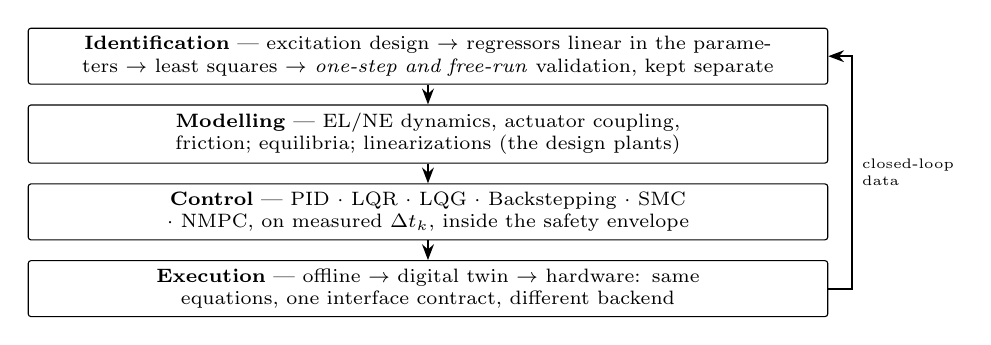
\begin{tikzpicture}[
  node distance=2.5mm,
  blk/.style={draw, rounded corners=1pt, align=center, font=\scriptsize, inner sep=3pt, text width=0.82\columnwidth},
  arr/.style={-{Stealth[length=2mm]}, thick}
]
\node[blk] (id) {\textbf{Identification} --- excitation design $\to$ regressors linear in the parameters $\to$ least squares $\to$ \emph{one-step and free-run} validation, kept separate};
\node[blk, below=of id] (mod) {\textbf{Modelling} --- EL/NE dynamics, actuator coupling, friction; equilibria; linearizations (the design plants)};
\node[blk, below=of mod] (ctl) {\textbf{Control} --- PID $\cdot$ LQR $\cdot$ LQG $\cdot$ Backstepping $\cdot$ SMC $\cdot$ NMPC, on measured $\Delta t_k$, inside the safety envelope};
\node[blk, below=of ctl] (exe) {\textbf{Execution} --- offline $\to$ digital twin $\to$ hardware: same equations, one interface contract, different backend};
\draw[arr] (id) -- (mod);
\draw[arr] (mod) -- (ctl);
\draw[arr] (ctl) -- (exe);
\draw[arr] (exe.east) -- ++(3mm,0) |- node[font=\tiny, pos=0.25, right, align=left] {closed-loop\\ data} (id.east);
\end{tikzpicture}
\caption{The workflow every platform in this series follows: identification feeds modelling, modelling feeds the controller suite, and all stages run unchanged across the three execution targets; closed-loop records return to identification.}
\label{fig:workflow}
\end{figure}
Equation \eqref{eq:armdyn} is linear in the \emph{base inertial parameters} $\pi$ (the identifiable regrouping of link masses, first moments, inertias, friction, and reflected terms):
\begin{equation}
Y(q, \dot q, \ddot q)\,\pi = \tau,
\end{equation}
with $\tau$ from measured currents ($\hat\tau = N k_t i$ through gear efficiency $\eta(N)$ --- the efficiency uncertainty is the accuracy floor). Protocol: E1) \emph{gravity vector} from quasi-static postures spanning the elevation angles ($\ddot q \approx \dot q \approx 0$ isolates $G(q)$, linear in mass moments); E2) \emph{friction} per joint from constant-velocity sweeps in both directions; E3) \emph{excitation trajectories} --- periodic joint trajectories optimizing the regressor condition number (finite Fourier series with joint-limit and velocity constraints), least squares for the full $\pi$; E4) payload identification from the change in $\pi$ of the last link (linear). Validation: torque prediction on held-out trajectories, one-step and free-run (torque replay vs.\ motion replay) reported separately.

%====================================================================
\section{Control Suite}
Current mode is assumed (torque-assignable) except where noted; all discrete updates on measured $\Delta t_k$; commands respect the current, velocity, and thermal clamps.

\subsection{PID with gravity compensation}
Per joint,
\begin{equation}
\tau = K_p e + K_i\!\int e\,dt + K_d\,\hat{\dot e} + \hat G(q),
\end{equation}
diagonal gains; $\hat G$ from E1 converts the gravity-dominated plant into a near-double-integrator per joint --- \emph{the} decisive model injection on this class of arm (global asymptotic stability of PD+gravity compensation for regulation follows from the standard Lyapunov argument with $V = \tfrac12\dot q^{\!\top}M\dot q + \tfrac12 e^{\!\top}K_p e$). In position mode, the same structure runs inside the servos; the outer loop then shapes setpoints only.

\subsection{LQR / LQG}
Linearize \eqref{eq:armdyn} about a working configuration $q_0$: $M_0\ddot{\tilde q} + F_{v}\dot{\tilde q} + K_G\tilde q = \tilde\tau$ with the gravity stiffness $K_G = \partial G/\partial q|_{q_0}$ (destabilizing sign for elevated postures); state $[\tilde q^{\!\top}, \dot{\tilde q}^{\!\top}]^{\!\top}\in\mathbb R^8$, CARE gain gain-scheduled over the workspace grid. LQG adds the Kalman filter over encoder quantization and bus-delay-augmented measurements; separation nominal, delay margin checked against the bus period.

\subsection{Computed torque / backstepping}
Exact feedback linearization is available (fully actuated):
\begin{equation}
\tau = M(q)\bigl(\ddot q_d + K_d\dot e + K_p e\bigr) + C(q,\dot q)\dot q + G(q),
\label{eq:ct}
\end{equation}
yielding decoupled error dynamics $\ddot e + K_d\dot e + K_p e = M^{-1}\tilde Y\tilde\pi$, with the residual bounded by the identification error. Backstepping delivers the same law with a Lyapunov construction that extends to the servo current lag: $z_1 = e$, $z_2 = \dot e + c_1 z_1$, $V = \tfrac12 z_1^{\!\top}z_1 + \tfrac12 z_2^{\!\top}M z_2$, $\dot V = -c_1\|z_1\|^2 - c_2 z_2^{\!\top}z_2$ using skew symmetry --- and a third stage through $L_a\dot i$ when the current loop is slow enough to matter.

\subsection{Sliding mode}
$s = \dot e + \Lambda e$; $\tau = M(\ddot q_d + \Lambda\dot e) + C\dot q + G - K_s\sat(s/\phi)$ (Slotine--Li form), $K_s$ sized to $\|\tilde Y\tilde\pi\|_\infty$ from the identification residuals plus payload uncertainty; boundary layer above the encoder-rate noise. The adaptive variant $\dot{\hat\pi} = -\Gamma Y^{\!\top}s$ exploits the same regressor as identification --- the mathematical kinship between E3 and adaptive control made explicit.

\subsection{NMPC}
Receding horizon on \eqref{eq:armdyn} (RK4), cost over joint or Cartesian error plus torque effort, constraints: joint limits, velocity/current clamps, \emph{Cartesian keep-out sets} (table, self-collision) as state constraints, and the thermal continuous-torque budget as an integral constraint --- the formulation in which workspace safety and actuator physics enter the same optimization. Real-time reductions as on our other platforms; for pick-and-place, the linear time-varying MPC about the planned trajectory is the standard efficient variant.

%====================================================================
\section{Execution Modes and Conclusion}
Offline: \eqref{eq:armdyn} with servo-mode, bus-latency, and quantization models injectable; digital twin: the vendor virtual QArm under the same joint command/measurement contract (position-mode parity first, current-mode where exposed); hardware under the gravity-safe stop discipline. The mathematics above --- reflected-inertia actuation physics, closed-form kinematics with singularity handling, structurally exact Euler--Lagrange dynamics linear in identifiable parameters, and the six-controller suite ordered by what gravity dominance actually rewards --- constitute the platform's single source of truth across all three targets.

\bibliographystyle{IEEEtran}
\begin{thebibliography}{9}
\bibitem{siciliano2009} B.~Siciliano, L.~Sciavicco, L.~Villani, and G.~Oriolo, \emph{Robotics: Modelling, Planning and Control}. Springer, 2009.
\bibitem{spong2006} M.~W. Spong, S.~Hutchinson, and M.~Vidyasagar, \emph{Robot Modeling and Control}. Wiley, 2006.
\bibitem{slotine1991} J.-J.~E. Slotine and W.~Li, \emph{Applied Nonlinear Control}. Prentice Hall, 1991.
\bibitem{swevers2007} J.~Swevers, W.~Verdonck, and J.~De Schutter, ``Dynamic model identification for industrial robots,'' \emph{IEEE Control Syst. Mag.}, 2007.
\bibitem{quanser_qarm} Quanser Consulting Inc., \emph{QArm User Manual}, Markham, ON, Canada.
\bibitem{khalil2002} H.~K. Khalil, \emph{Nonlinear Systems}, 3rd ed. Prentice Hall, 2002.
\bibitem{rawlings2017} J.~B. Rawlings, D.~Q. Mayne, and M.~Diehl, \emph{Model Predictive Control}, 2nd ed. Nob Hill, 2017.
\end{thebibliography}

\end{document}
